% !TeX root = definitions_of_asymptotic_cones.tex
\documentclass[a4paper,11pt]{jsarticle}

% 英文化
\usepackage[english]{babel}
% 数式
\usepackage{amsmath}
\usepackage{amsfonts}
\usepackage{amsthm}
\usepackage{amssymb}
\usepackage{bm}
\usepackage{mathtools}
% 画像
\usepackage[dvipdfmx]{graphicx}
% 箇条書き
\usepackage{enumitem}

% 枠付き文章
\usepackage{ascmac}

\newcommand{\QUOTEBOX}[1]{\begin{center}\fbox{\begin{minipage}{.8\textwidth}{#1}\end{minipage}}\end{center}}
\newcommand{\DEFINITION}[2]{\begin{itembox}[l]{\underline{Definition {#1} }}{#2}\end{itembox}}
\newcommand{\PROPOSITION}[2]{\begin{itembox}[l]{\underline{Proposition {#1} }}{#2}\end{itembox}}
\newcommand{\REMARK}[2]{\begin{itembox}[l]{\underline{Remark {#1} }}{#2}\end{itembox}}

\newcommand{\NaturalNumberSet}{\mathbb{N}}
\newcommand{\RealNumberSet}{\mathbb{R}}
\newcommand{\NDemenstionalRealEuclidianSpace}{\mathbb{R}^n}


\SetLabelAlign{Center}{\hfil#1\hfil}
\SetLabelAlign{CenterWithParen}{\hfil(\makebox[1.0em]{#1})\hfil}
\SetLabelAlign{CenterWithParen2}{\hfil(\makebox[1.5em]{#1})\hfil}


\renewcommand{\theenumi}{\roman{enumi}}
\renewcommand{\labelenumi}{(\theenumi)}
\renewcommand{\theenumii}{\theenumi-\alph{enumii}}
\renewcommand{\labelenumii}{(\theenumii)}

\begin{document}

\title{
  2 Asymptotic Cones and Functions \\
  \large 2.1 Definition of Asymptotic Cones}
\author{Ryota Iwamoto}
\date{\today}
\maketitle

We use the book; Asymptotic Cones and Functions in Optimization and Variational Inequalities (author: A.AUSLENDER and M.TEBOULLE), pp.25-31.

\QUOTEBOX{
  The set of natural numbers is denoted by $\NaturalNumberSet$, so that $k \in \NaturalNumberSet$ means $k = 1,2, \dots .$ A sequence $\{x_k\}_{k \in \NaturalNumberSet}$ or simply $\{x_k\}$ in $\NDemenstionalRealEuclidianSpace$ is said to converge to $x$ if $\left\lVert x_k - x\right\rVert \rightarrow 0$ as $k \rightarrow \infty$, and this will be indicated by the notation $x_k \rightarrow x$ or $x = \lim_{k \to \infty} x_k$. We say that $x$ is a cluster point of $\{x_k\}$ if some subsequence converge to $x$. Recall that every bounded sequence in $\NDemenstionalRealEuclidianSpace$ converges to $x$ if and only if it is bounded and has $x$ as its unique cluster point.

  Let $\{x_k\}$ be a sequence in $\NDemenstionalRealEuclidianSpace$. We are interested in knowing how to handle convergence properties, we are led to consider direction $d_k \coloneqq x_k\left\lVert x_k\right\rVert^{-1}$ with $x_k \neq 0$, $k \in \NaturalNumberSet$. From classical analysis, the Bolzano-Weierstrass theorem implies that we can extract a convergent subsequence $d = \lim_{k \in K} d_k$, $K \subset \NaturalNumberSet$, with $d \neq 0$. Now suppose that the sequence $\{x_k\} \subset \NDemenstionalRealEuclidianSpace$ is such that $\left\lVert x_k \right\rVert \rightarrow + \infty$. Then
  \begin{equation}
    \exists t_k \coloneqq \left\lVert x_k \right\rVert, k \in K \subset \NaturalNumberSet, \text{ such that } \lim_{k \in K} t_k = + \infty \:\text{and}\: \lim_{k \in K} \frac{x_k}{t_k} = d. \notag
  \end{equation}
  This leads us to introduce the following concepts.
}

\DEFINITION{2.1.1}{
  A sequence $\{x_k\} \subset \RealNumberSet$ is said to converge to a direction $d \in \NDemenstionalRealEuclidianSpace$ if
  \begin{equation}
    \exists \{t_k\}, \:with\: t_k \rightarrow + \infty \:\text{ such that }\: \lim_{k \to \infty} \frac{x_k}{t_k} = d. \notag
  \end{equation}
}

\DEFINITION{2.1.2}{
  Let $C$ be a nonempty set in $\NDemenstionalRealEuclidianSpace$. Then the asymptotic cone of the set $C$, denoted by $C_{\infty}$, is the set of vectors $d \in \NDemenstionalRealEuclidianSpace$ that are limits in direction of the sequences $\{x_k\} \subset C$, namely
  \begin{equation}
    C_{\infty} = \{d \in \NDemenstionalRealEuclidianSpace \:|\: \exists t_k \rightarrow + \infty , \exists x_k \in C \:\text{ with }\: \lim_{k \to \infty} \frac{x_k}{t_k} = d \}. \notag
  \end{equation}
}

\QUOTEBOX{
  From the definition we immediately deduce the following elementary facts.
}

\PROPOSITION{2.1.1}{
  Let $C \subset \NDemenstionalRealEuclidianSpace$ be nonempty. Then:
  \begin{enumerate}[label=\roman*,align=CenterWithParen]
    \item $C_{\infty}$ is a closed cone.
    \item $(\text{cl}\:C)_{\infty} = C_{\infty}$.
    \item If $C$ is a cone, then $C_{\infty} = \text{cl}\:C$.
  \end{enumerate}
}

\begin{proof}
  We will prove each part separately.
  \begin{enumerate}[label=\roman*,align=CenterWithParen]
    \item $C_{\infty}$ is a closed cone.

      We need to show two propositions: (i-a) $C_{\infty}$ is a cone and (i-b) $C_{\infty}$ is a closed set.

      \begin{enumerate}[label=i-\alph*,align=CenterWithParen]
        \item We show that $C_{\infty}$ is a cone, that is, $\forall \alpha \geq 0, d \in C_{\infty}, \alpha d \in C_{\infty}$.

        Since $0$ is a element of $C_{\infty}$, it is clear in the case of $\alpha = 0$.

        ($\because$ Since $C$ is nonempty, we can take a element $x_0$ from $C$. In addition we take a sequence $\{t_k\}_{k=1}^{\infty}$ with $t_k \rightarrow + \infty$ as $k \rightarrow \infty$. Of course this sequence exists, for example $t_k \coloneqq k$. By using $t_k \coloneqq k$ and $x_k \coloneqq x_0$, we can obtain $0$ as the limit. Hence $0$ is a element of $C_{\infty}$.)

        Also we consider the other case $\alpha > 0$. To prove that $C_{\infty}$ is a cone, we take a any direction $d$ from $C_{\infty}$. Since d is a element of $C_{\infty}$,

        \begin{equation}
          \exists t_k \rightarrow + \infty , \exists x_k \in C \:\text{ with }\: \lim_{k \to \infty} \frac{x_k}{t_k} = d. \notag
        \end{equation}

        Then we define a sequence $\{t'_k\}_{k=1}^{\infty} \coloneqq \frac{t_k}{\alpha}$, exactly whose limit becomes $+\infty$ as $k \rightarrow \infty$. Accordingly there exist $t'_k \rightarrow + \infty$ and $x_k \in C$ with

        \begin{equation}
          \lim_{k \to \infty} \frac{x_k}{t'_k} = \lim_{k \to \infty} \alpha \cdot \frac{x_k}{t_k} = \alpha d. \notag
        \end{equation}

        This means $d \in C_{\infty}$.

        By these results, we can get $\forall \alpha \geq 0, d \in C_{\infty}, \alpha d \in C_{\infty}$.

        Therefore $C_{\infty}$ is a cone.

        \item We show that $C_{\infty}$ is a closed set. In order to prove closeness, we consider convergency of a sequence of $C_{\infty}$. First we take a sequence $\{d_k\}_{k=1}^{\infty} \subset C_{\infty}$ with $d_k \rightarrow d$ as $k \rightarrow \infty$ for some $d$. Then we don't forget that $d \in C_{\infty}$ is our goal.

        For each $k \in \NaturalNumberSet$,

        \begin{equation}
          \exists \{x_k^{(n)}\}_{n=1}^{\infty} \subset C \:\text{and}\: \{t_k^{(n)}\}_{n=1}^{\infty} \:\text{with}\: t_k^{(n)} \rightarrow \infty \:\text{as}\: n \rightarrow \infty. \notag
        \end{equation}

        The below figure represents $x_k^{(n)}$ and $t_k^{(n)}$.
        \medskip

        Figure:

        \medskip

        \begin{center}
          \large
          \begin{tabular}{|c|c|c|c|c|c|c|} \hline
            $k$ \textbackslash $n$ & $1$ & $2$ & $\cdots$ & $m$ & $\cdots$ & limit \\ \hline
            $1$ & $x_1^{(1)}$, $t_1^{(1)}$ & $x_1^{(2)}$, $t_1^{(2)}$ & $\cdots$ & $x_1^{(m)}$, $t_1^{(m)}$ & $\cdots$ & $d_{1}$ \\
            $2$ & $x_2^{(1)}$, $t_2^{(1)}$ & $x_2^{(2)}$, $t_2^{(2)}$ & $\cdots$ & $x_2^{(m)}$, $t_2^{(m)}$ & $\cdots$ & $d_{2}$ \\
            $\vdots$ & $\vdots$ & $\vdots$ & $\ddots$ & $\vdots$ & $\vdots$ & $\vdots$ \\
            $m$ & $x_m^{(1)}$, $t_m^{(1)}$ & $x_m^{(2)}$, $t_m^{(2)}$ & $\cdots$ & $x_m^{(m)}$, $t_m^{(m)}$ & $\cdots$ & $d_{m}$ \\
            $\vdots$ & \multicolumn{6}{|c|}{$\vdots$} \\ \hline
          \end{tabular}
        \end{center}

        \medskip

        Then we define

        \begin{equation}
          x_m \coloneqq x_m^{(m)} \:\text{and}\: t_m \coloneqq t_m^{(m)}. \notag
        \end{equation}

        By the definition of convergence of a sequence,

        \begin{equation}
          \begin{split}
            \forall \epsilon &> 0, \exists \bar{m} \in \NaturalNumberSet \:s.t.\: \forall m \geq \bar{m}, ||d_m -d|| < \frac{\epsilon}{2}, \text{and} \\
            \forall \epsilon &> 0, \exists \hat{m} \in \NaturalNumberSet \:s.t.\: \forall m \geq \hat{m}, ||\frac{x_m}{t_m} -d_m|| < \frac{\epsilon}{2}. \notag
          \end{split}
        \end{equation}

        Also, we let $\tilde{m} \coloneqq \:\text{max}\:\{\bar{m},\hat{m}\} \in \NaturalNumberSet$. By using triangle inequality,

        \begin{equation}
            \forall \epsilon > 0, \exists \tilde{m} \in \NaturalNumberSet \:s.t.\: \forall m \geq \bar{m}, ||\frac{x_m}{t_m} -d|| < \epsilon.\notag
        \end{equation}

        ($\because ||\frac{x_m}{t_m} -d|| \leq ||\frac{x_m}{t_m} - d_m|| + ||d_m - d|| < \epsilon.\notag $.)

        Therefore $c_{\infty}$ is a closed set.
      \end{enumerate}
      Then (i)'s proof is completed.
    \item $(\text{cl}\:C)_{\infty} = C_{\infty}$.

    We need to show two relations: (ii-a) $(\text{cl}\:C)_{\infty} \supset C_{\infty}$ (ii-b) $(\text{cl}\:C)_{\infty} \subset C_{\infty}$.

      \begin{enumerate}[label=ii-\alph*,align=CenterWithParen2]
        \item We show that $C_{\infty}$ is included in $(\text{cl}\:C)_{\infty}$. However it is clear from the definition of asymptotic cone.

        \item We show that $(\text{cl}\:C)_{\infty} \subset C_{\infty}$. In order to prove that a element of $(\text{cl}\:C)_{\infty}$ satisfies the asymptotic cone's relation, we consider convergency of a sequences of $(\text{cl}\:C)_{\infty}$ and $\text{cl}\:C$. First we take any $d \in (\text{cl}\:C)_{\infty}$ which satisfies

        \begin{equation}
          \exists t_k \rightarrow + \infty , \exists x_k \in \text{cl}\:C \:\text{ with }\: \lim_{k \to \infty} \frac{x_k}{t_k} = d. \notag
        \end{equation}

        For each $k \in \NaturalNumberSet$,

        \begin{equation}
          \exists \{y_k^{(n)}\}_{n=1}^{\infty} \subset C \:\text{with}\: y_k^{(n)} \rightarrow x_k \:\text{as}\: n \rightarrow \infty. \notag
        \end{equation}

        The below figure represents $y_k^{(n)}$.
        \medskip

        Figure:

        \medskip

        \begin{center}
          \large
          \begin{tabular}{|c|c|c|c|c|c|c|} \hline
            $k$ \textbackslash $n$ & $1$ & $2$ & $\cdots$ & $m$ & $\cdots$ & limit \\ \hline
            $1$ & $y_1^{(1)}$ & $y_1^{(2)}$ & $\cdots$ & $y_1^{(m)}$ & $\cdots$ & $x_{1}$ \\
            $2$ & $y_2^{(1)}$ & $y_2^{(2)}$ & $\cdots$ & $y_2^{(m)}$& $\cdots$ & $x_{2}$ \\
            $\vdots$ & $\vdots$ & $\vdots$ & $\ddots$ & $\vdots$ & $\vdots$ & $\vdots$ \\
            $m$ & $y_m^{(1)}$ & $y_m^{(2)}$ & $\cdots$ & $y_m^{(m)}$ & $\cdots$ & $x_{m}$ \\
            $\vdots$ & \multicolumn{6}{|c|}{$\vdots$} \\ \hline
          \end{tabular}
        \end{center}

        \medskip

        Then we define

        \begin{equation}
          y_m \coloneqq y_m^{(m)}. \notag
        \end{equation}

        By the definition of convergence of a sequence,

        \begin{equation}
          \begin{split}
            \forall \epsilon &> 0, \exists \bar{m} \in \NaturalNumberSet \:s.t.\: \forall m \geq \bar{m}, ||d_m -d|| < \frac{\epsilon}{2}, \\
            \forall \epsilon &> 0, \exists \hat{m} \in \NaturalNumberSet \:s.t.\: \forall m \geq \hat{m}, ||y_m^{m} -x_m|| < \frac{\sqrt{\epsilon}}{2}, \text{and} \\
            \forall \epsilon &> 0, \exists \tilde{m} \in \NaturalNumberSet \:s.t.\: \forall m \geq \tilde{m}, |\frac{1}{t_m}| < \sqrt{\epsilon}. \notag
          \end{split}
        \end{equation}

        Also, we let $m_0 \coloneqq \:\text{max}\:\{\bar{m},\hat{m}, \tilde{m}\} \in \NaturalNumberSet$. By using triangle inequality,

        \begin{equation}
            \forall \epsilon > 0, \exists m_0 \in \NaturalNumberSet \:s.t.\: \forall m \geq \bar{m}, ||\frac{y_m}{t_m} -d|| < \epsilon.\notag
        \end{equation}

        ($\because ||\frac{y_m}{t_m} -d|| \leq \frac{1}{|t_m|} \cdot ||y_m - d_m|| + ||\frac{y_m}{t_m} - d|| < \epsilon. \notag $)

        Therefore $(\text{cl}\:C)_{\infty} \subset C_{\infty}$.

      \end{enumerate}
      Then (ii)'s proof is also completed.
    \item If $C$ is a cone, then $C_{\infty} = \text{cl}\:C$.

    We need to show two relations: (iii-a) $C_{\infty} \subset \text{cl}\:C$ and (iii-b) $C_{\infty} \supset  \text{cl}\:C$.

    \begin{enumerate}[label=iii-\alph*,align=CenterWithParen2]
      \item We take any direction $d \in C_{\infty}$ which satisfies

      \begin{equation}
        \exists t_k \rightarrow + \infty , \exists x_k \in C \:\text{ with }\: \lim_{k \to \infty} \frac{x_k}{t_k} = d. \notag
      \end{equation}

      Let $d_k \coloneqq \frac{x_k}{t_k}$ (with $d_k \rightarrow d$ as $k \rightarrow \infty$). Since $C$ is a cone,

      \begin{equation}
        d_k = \frac{1}{t_k} \cdot x_k \in C. \notag
      \end{equation}

      Due to $d_k \in C$, the limit of $d_k$ is a element of $\text{cl}\:C$, i.e., $d \in \text{cl}\:C$.

      Therefore $C_{\infty} \subset \text{cl}\:C$.

      \item We take any $d \in \text{cl}\:C$ and show $d \in C_{\infty}$, that is,

      \begin{equation}
        \exists t_k \rightarrow + \infty , \exists x_k \in C \:\text{ with }\: \lim_{k \to \infty} \frac{x_k}{t_k} = d. \notag
      \end{equation}

      By $d \in \text{cl}\:C$,

      \begin{equation}
        \exists \{d_k\}_{k=1}^{\infty} \in C \:\text{with}\: d_k \rightarrow d \:\text{as}\: k \rightarrow \infty, \notag
      \end{equation}

      in other words,

      \begin{equation}
        \lim_{k \to \infty} d_k = d. \notag
      \end{equation}

      We define $y_k = k \cdot d_k$ and $s_k = k$ for each $k$. Since $d_k \in C$ and $C$ is a cone, $y_k$ is also a element of $C$.

      There exist $\{s_k\}_{k=1}^{\infty}$ with $s_k \rightarrow \infty$ as $k \rightarrow \infty$ and $\{y_k\}_{k=1}^{\infty} \subset C$ such that

      \begin{equation}
        \lim_{k \to \infty} \frac{y_k}{s_k} = \lim_{k \to \infty} d_k = d. \notag
      \end{equation}

      As $d$ is a element of $C_{\infty}$, therefore $C_{\infty} \supset  \text{cl}\:C$.

    \end{enumerate}

  \end{enumerate}
\end{proof}

\QUOTEBOX{
  The importance of the asymptotic cone is revealed by the following key property, which is a immediate consequence of its definition.
}

\PROPOSITION{2.1.2}{
  A set $C \subset \NDemenstionalRealEuclidianSpace$ is bounded if and only if $C_{\infty} = \{0\}$.
}

\begin{proof}
  We show that:

  \begin{enumerate}[label=\roman*,align=CenterWithParen]
    \item a set $C \subset \NDemenstionalRealEuclidianSpace$ is bounded $\Rightarrow $ $C_{\infty} = \{0\}$, and
    \item a set $C \subset \NDemenstionalRealEuclidianSpace$ is unbounded $\Rightarrow $ $C_{\infty} \ne \{0\}$.
  \end{enumerate}

  \begin{enumerate}[label=\roman*,align=CenterWithParen]
    \item By Proposition 2.1.1 (i), $0 \in C_{\infty}$. Also, by the assumption $C$ is bounded,

    \begin{equation}
      \exists r > 0, \forall x_k \in C \:\text{where}\: k \in \NaturalNumberSet,  \left\lVert x_k \right\rVert \leq r. \notag
    \end{equation}

    For any sequence $\{t_k\}_{k=1}^{\infty}$ such that $t_k \rightarrow \infty$ as $k \rightarrow \infty$,

    \begin{equation}
      \lim_{k \to \infty} \frac{x_k}{t_k} = 0. \notag
    \end{equation}

    Thus the limit becomes only 0 for any $\{x_k\}_{k=1}^{\infty} \subset C$ and $\{t_k\}_{k=1}^{\infty}$ with $t_k \rightarrow \infty$ as $k \rightarrow \infty$.

    Therefore if $C$ is bounded then $C_{\infty} = \{0\}$.

    \item If $C$ is unbounded, then there exists a sequence $\{x_k\} \subset C$ with $x_k \ne 0$, $\forall k \in \NaturalNumberSet$, such that $t_k \coloneqq \left\lVert t_k \right\rVert \rightarrow \infty$ and thus the vectors $d_k = t_k^{-1} x_k \in \{ d \:\colon\: \left\lVert d\right\rVert = 1 \}$.

    By the Bolzano-Weierstrass, we can extract a subsequence of $\{d_k\}$ such that $\lim_{k \in K} d_k = d$, $K \subset \NaturalNumberSet$, and with $\left\lVert d \right\rVert = 1$. This nonzero vector $d$ is an element of $C_{\infty}$ by Definition 2.1.2, a contradiction.
  \end{enumerate}
\end{proof}

Figure:

Why do we take a subsequence of $\{d_k\}$?

\begin{center}
  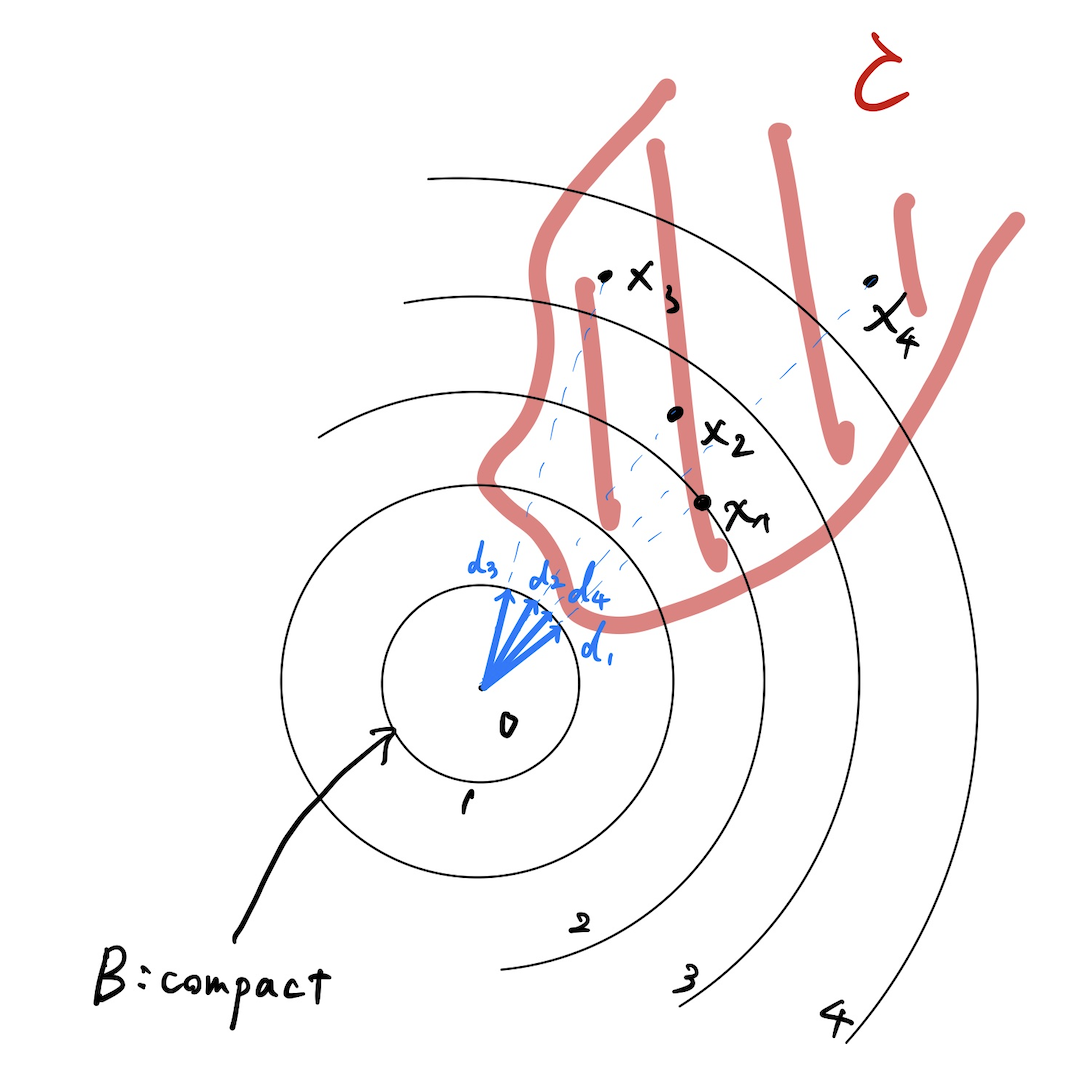
\includegraphics[width=8cm]{figures/asymptotic_cones_in_the_case_of_unbounded.png}
\end{center}

\QUOTEBOX{
  Associated with the asymptotic cone $C_{\infty}$ is the following related concept, which will help us in simplifying the definition of $C_{\infty}$ in the particular case where $C \in \NDemenstionalRealEuclidianSpace$ is assumed convex.
}

\DEFINITION{2.1.3}{
  Let $C \in \NDemenstionalRealEuclidianSpace$ be nonempty and define
  \begin{equation}
    C_{\infty}^1 = \{d \in \NDemenstionalRealEuclidianSpace \:|\: \forall t_k \rightarrow + \infty , \exists x_k \in C \:\text{ with }\: \lim_{k \to \infty} \frac{x_k}{t_k} = d \}. \notag
  \end{equation}
  We say that C is asymptotically regular if $C_{\infty} = C_{\infty}^1$
}

Remark: A set $D=\{(x,y) \in \RealNumberSet_{+} \times \RealNumberSet_{+} \:|\: y= e^x - 1\}$ is not asymptotically regular.

\PROPOSITION{2.1.3}{
  Let $C$ be a nonempty convex set in $\NDemenstionalRealEuclidianSpace$. Then $C$ is asymptotically regular.
}

\begin{proof}
  The inclusion $C_{\infty}^{1} \subset C_{\infty}$ clearly holds from the definition of $C_{\infty}^{1}$ and $C_{\infty}$, respectively. Let $d \in C_{\infty}$. Then $\exists \{x_k\} \in C$, $\exists s_k \rightarrow \infty$ such that $d = \lim_{k \to \infty} s^{-1} x_k$. Let $x \in C$ and define $d_k = s^{-1}(x_k - x)$. Then we have

  \begin{equation}
    d = \lim_{k \to \infty} d_k, x + s_k d_k \in C. \notag
  \end{equation}

  $\because$ $x_k = x + s_k d_k \in C$.

  Now note that an arbitrary sequence such that $\lim_{k \to \infty} t_k = +\infty$. For any fixed $m \in \NaturalNumberSet$, there exists $k(m)$ with $\lim_{m \to \infty} k(m) = +\infty$ such that $t_m \leq s_{k(m)}$, and since $C$ is convex, we have $x'_m = x + t_m + t_m d_{m(k)} \in C$. Hence, $d = \lim_{m \to \infty} t_m^{-1} x'_m$, showing that $d \in C_{\infty}^1$.

\end{proof}

Figure:

Why should we consider $k(m)$ with $\lim_{m \to \infty} k(m) = +\infty$ such that $t_m \leq s_{k(m)}$?

If $\{s_k\} = 1,2,3,7,8,9,13, \cdots$ and $\{t_k\} = 1,3,4,6,8,10,11, \cdots$, then we can get

\begin{equation}
  \{k(m)\} = 1,3,4,5,6,6, \cdots. \notag
\end{equation}

\begin{center}
  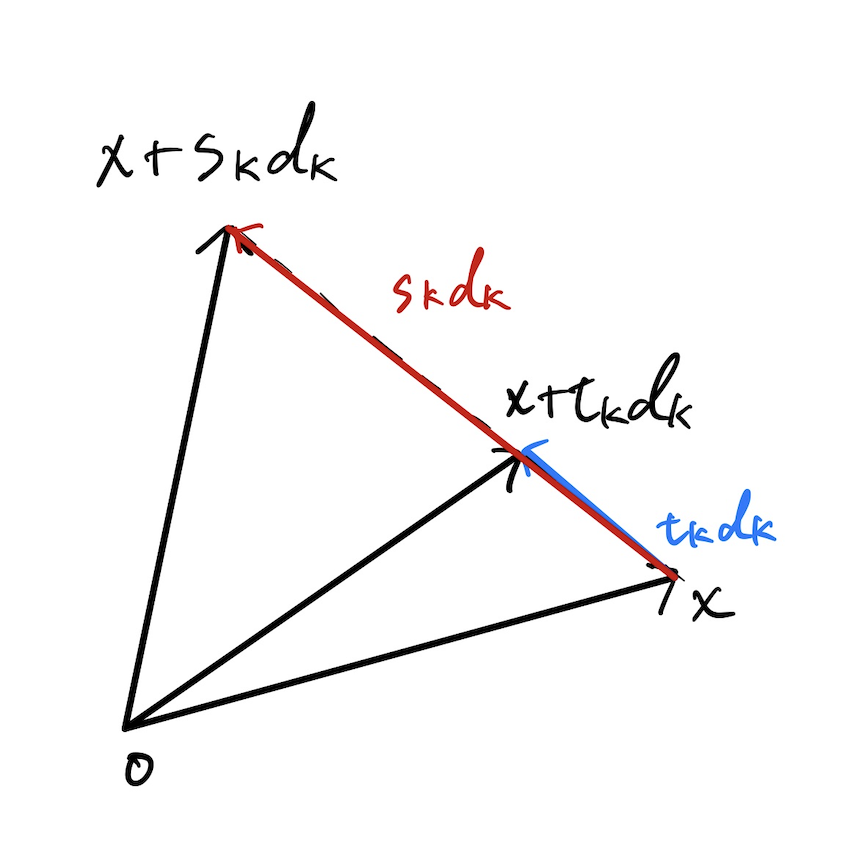
\includegraphics[width=5cm]{figures/asymptotically_regular_associated_with_convex.png}
\end{center}

\QUOTEBOX{
  We note that a set can be nonconvex, yet asymptotically regular Indeed, consider, for example, sets definition by $C \coloneqq S + K$, with $S$ compact and $K$ a closed convex cone. Then clearly $C$ is not necessarily convex, but it can be easily seen that $C_{\infty} = C_{\infty}^1$.
}
\REMARK{2.1.1}{
  Note that the definitions of $C_{\infty}$ and $C_{\infty}^1$ are related to the theory of set convergence of Painleve-Kuratowski. Indeed, for a family $\{C_t\}_{t>0}$ of subsets of $\NDemenstionalRealEuclidianSpace$, the outer limit as $t \rightarrow + \infty$ is the set.

  \begin{equation}
    \limsup_{t \to +\infty} C_t = \{x \:|\: \liminf_{t \to +\infty} d(x, C_t) = 0\}, \notag
  \end{equation}

  while the inner limit as $t \rightarrow +\infty$ is the set

  \begin{equation}
    \liminf_{t \to +\infty} C_t = \{x \:|\: \limsup_{t \to +\infty} d(x, C_t) = 0\}, \notag
  \end{equation}

  It can then be verified that the corresponding asymptotic cones can be written as

  \begin{equation}
    C_{\infty} = \limsup_{t \to +\infty} t^{-1} C,\:\: C_{\infty}^1  = \liminf_{t \to +\infty} t^{-1} C. \notag
  \end{equation}

}

\end{document}
